\documentclass[10pt]{article}
\usepackage[polish]{babel}
\usepackage[utf8]{inputenc}
\usepackage[T1]{fontenc}
\usepackage{graphicx}
\usepackage[export]{adjustbox}
\graphicspath{ {./images/} }

\title{Akademia \\
 Pomorska \\
 w Stupsku }

\author{}
\date{}


\begin{document}
\maketitle
\begin{center}

\includegraphics[max width=\textwidth]{2024_11_21_7622132ecf434143f224g-1}
\end{center}

\begin{center}
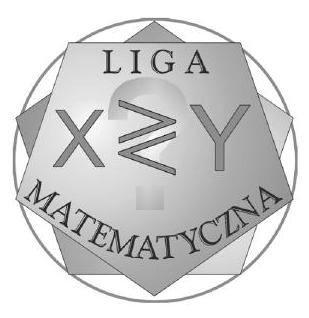
\includegraphics[max width=\textwidth]{2024_11_21_7622132ecf434143f224g-1(1)}
\end{center}

\section*{LIGA MATEMATYCZNA im. Zdzisława Matuskiego \\
 PÓŁFINAŁ 27 kwietnia 2021 \\
 SZKOŁA PODSTAWOWA \\
 klasy IV - VI}
\section*{ZADANIE 1.}
Ania ma siedem monet dwuzłotowych, a Bartek ma osiem monet pięciozłotowych. Jaką najmniejszą liczbę monet muszą wymienić między sobą, aby mieć równe kwoty?

\section*{ZADANIE 2.}
Znajdź najmniejszą liczbę naturalną, która w zapisie dziesiętnym ma tylko 0 i 1 oraz jest podzielna przez 45. Odpowiedź uzasadnij.

\section*{ZADANIE 3.}
Za pięć lat dwie siostry i dwaj bracia będą mieli razem 60 lat. Wyznacz łączny ich wiek za piętnaście lat.

\section*{ZADANIE 4.}
Tort trzywarstwowy łącznie z paterą, na której stoi, ma 70 cm wysokości. Tort jednowarstwowy łącznie z taką samą paterą, ma wysokość 36 cm . W obu tortach każda warstwa ma tę samą wysokość. Wyznacz wysokość patery.

\section*{ZADANIE 5.}
Prostokąt podzielono na dziewięć mniejszych prostokątów. Obwody trzech z nich podano na rysunku. Oblicz obwód dużego prostokąta.

\begin{center}
\begin{tabular}{|l|l|l|}
\hline
20 &  &  \\
\hline
 &  & 15 \\
\hline
 & 9 &  \\
\hline
\end{tabular}
\end{center}


\end{document}